\documentclass{article}

\usepackage{minted}
\usepackage[most]{tcolorbox}
\usepackage{geometry}
\usepackage{enumitem}
\usepackage{hyperref}
\usepackage{hyperref}
\usepackage[parfill]{parskip}
\usepackage{wrapfig}
\usepackage{accsupp}

\geometry{margin=0.8in}
\definecolor{lightgreen}{rgb}{0.56, 0.93, 0.56}
\definecolor{moonstoneblue}{rgb}{0.45, 0.66, 0.76}
\definecolor{magenta}{rgb}{0.8,0.66,0.76}
\begin{document}
\begin{flushright}
\BeginAccSupp{}
Computational Biology ~\\
Tufts University Bio 35 ~\\
Fall 2021 ~\\ ~\\
\end{flushright}
\begin{center}{\textbf{\Large{Spotlight 2: Charles Chiu}}}\end{center}

\begin{wrapfigure}{L}{0.11\textwidth}
\begin{center}
 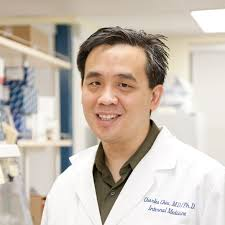
\includegraphics[width=0.1\textwidth]{images/charles-chiu.jpeg}
 \end{center}
\end{wrapfigure}
~\\ As part of our unit on pathogenic genes and virulence factors, we are going to explore the work of Charles Chiu. Charles Chiu's lab studies pathogens and develops computational tools for the identification of pathogens in genetic samples. He is a Professor at the University of California, San Francisco.

~\\
\vspace{-1em}

Please read the following articles about Charles Chiu's work: 
\begin{enumerate}
\item \texttt{\href{https://www.nytimes.com/2014/06/05/health/in-first-quick-dna-test-diagnoses-a-boys-illness.html}{https://www.nytimes.com/2014/06/05/health/in-first-quick-dna-test-diagnoses-a-boys-illness.html}}
\item \texttt{\href{https://www.eurekalert.org/pub_releases/2020-11/uoc--rtc111020.php}{https://www.eurekalert.org/pub\_releases/2020-11/uoc--rtc111020.php}}
\end{enumerate}

Also listen to the following short radio segment:
\begin{enumerate}
\item \texttt{\href{https://www.npr.org/sections/health-shots/2014/06/05/319210230/quick-dna-tests-crack-medical-mysteries-otherwise-missed}{https://www.npr.org/sections/health-shots/2014/06/05/319210230/quick-dna-tests-crack-medical...}}
\end{enumerate}

\subsubsection*{Written Assignment} 
After reading the articles about Charles Chiu, write
a reflection (max one page) on what you discovered. You might wish to address some of the following: 

\begin{enumerate}
\item What was most interesting to you in reviewing these resources?
\item What did you learn from these resources about computational approaches for detecting pathogens?
\item What new questions do you have after reviewing these resources?
\item What do these resources tell you about the types of people that do computational biology, or their motivations?
\end{enumerate}

\EndAccSupp{}
\end{document}
